% Generated by Listas/make_statements.py from pratica-lecture-05.md, item 12. Do not edit.
\textbf{Source.} Tadelis (2013), \emph{Game Theory: An Introduction}, Exercise 9.2 ``Centipedes Revisited'', p.~187 {[}PDF 206{]}. Answer in the source: none (the book prints no solutions; the preface says about half are on Princeton UP's website, not checked). Reproduced verbatim.



\begin{quote}

\textbf{Centipedes Revisited:} Two players are playing two consecutive games. First, they play the Centipede Game described in Figure 9.2. After the Centipede Game they play the following coordination game:



\pandocbounded{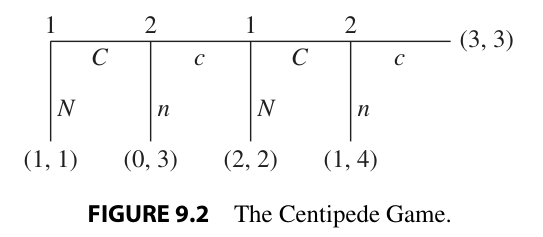
\includegraphics[keepaspectratio,alt={FIGURE 9.2 The Centipede Game}]{../figures/tadelis-9-2.png}}



{\def\LTcaptype{none} % do not increment counter

\begin{longtable}[]{@{}ccc@{}}

\toprule\noalign{}

Player 1 ~Player 2 & \(a\) & \(b\) \\

\midrule\noalign{}

\endhead

\bottomrule\noalign{}

\endlastfoot

\(A\) & 1, 1 & 0, 0 \\

\(B\) & 0, 0 & 3, 3 \\

\end{longtable}

}



\begin{enumerate}

\def\labelenumi{\alph{enumi}.}

\item

  What are the Nash equilibria of each stage-game?

\item

  How many pure strategies does each player have in the multistage game?

\item

  Find all the pure-strategy subgame-perfect equilibria with extreme discounting (\(\delta = 0\)). Be precise in defining history-contingent strategies for both players.

\item

  Now let \(\delta = 1\). Find a subgame-perfect equilibrium for the two-stage game in which the players receive the payoffs (2, 2) in the first stage-game.

\item

  What is the lowest value of \(\delta\) for which the subgame-perfect equilibrium you found in (d) survives?

\item

  For \(\delta\) greater than the value you found in (e), are there other outcomes of the first-stage Centipede Game that can be supported as part of a subgame-perfect equilibrium?

\end{enumerate}

\end{quote}

